\documentclass[tikz]{standalone}
\usepackage{pgfplots}
\pgfplotsset{compat=1.15}
\usepackage{mathrsfs}
\usetikzlibrary{arrows,calc}
\usepackage{tkz-euclide}

\usepackage{fp}
\pagestyle{empty}

\definecolor{AngleClr}{rgb}{0,0.39215686274509803,0}
\definecolor{ShapeClr}{rgb}{0.6,0.2,0}

\begin{document}

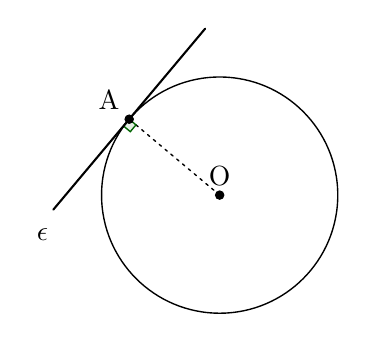
\begin{tikzpicture}[scale=.75]
\tkzSetUpLine[line width=1pt,color=black]
\tkzSetUpPoint[fill=black]

\tkzDefPoints{0/0/O,2/0/X,-3/-0.4/E}

\tkzDefPoint(140:2){A}

\tkzDrawSegments[line width=0.5pt,color=black,dashed,dash pattern=on 1pt off 1.75pt](O,A)

\tkzDrawCircle[color=black,line width=0.5pt](O,X)

\tkzDefLine[tangent at=A](O) \tkzGetPoint{h}

\tkzMarkRightAngle[line width=0.5pt, size=.15,color=AngleClr,fill=AngleClr,fill opacity=0.1](O,A,h)

\tkzDrawSegments[line width=0.75pt,color=black,add=2 and 1](A,h)

\tkzDrawPoints[size=3](A,O)
\tkzLabelPoint[above left](A){$\rm A$}
\tkzLabelPoint[above](O){$\rm O$}
\tkzLabelPoint(E){$\rm \epsilon$}

\end{tikzpicture}
\end{document}
